\documentclass{standalone}
\usepackage{tikz,ctex}
\usepackage{tikz-3dplot} % 2-1
\usepackage{unicode-math} % 2-5,4-1,4-2
\setmathfont{Fira Math Regular}
\setmainfont{Fira Sans}
\definecolor{background}{RGB}{239, 239, 239} % 4-5,6-2,6-5
\begin{document}
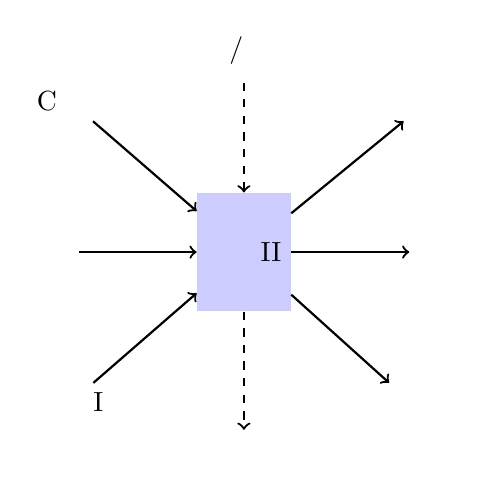
\begin{tikzpicture}[every pin edge/.style={thick},every pin/.style={pin distance=1.5cm}]
\node [fill=blue!20,minimum height = 1.5cm,
    pin={[pin edge={<-,dashed}]above:数学/离散数学},
    pin={[pin edge={->,dashed}]below:大学生程序设计竞赛},
    pin={[pin edge={<-}]above left:C语言程序设计},
    pin={[pin edge={<-}]left:数据结构},
    pin={[pin edge={<-}]below left:算法分析与设计I},
    pin={[pin edge={->}]above right:数据分析与可视化},
    pin={[pin edge={->}]right:最优化理论},
    pin={[pin edge={->}]below right:数据挖掘}] at (0,0) {算法分析与设计II};
\end{tikzpicture}
\end{document}